\chapter{TaCに関する資料}
\label{appTac}

%==============================================================================
\section{{\tac} CPUの概要}
TaCで使用できるデータの形式と,
メモリ空間,I/O空間,CPU内部のレジスタ等の構成を\figref{tacData}に示す.

\begin{myfig}{p}{TaC CPUの概要}{tacData}
  \includegraphics[scale=0.86,page=2]{Fig/TacInst-crop.pdf}
\end{myfig}

%==============================================================================
\section{メモリマップとI/Oマップ}
TaCのメモリマップ,I/Oマップ,
I/Oポート詳細を\figref{tacMap}
%と\figref{tacIO}
に示す.

\begin{myfig}{p}{TaCのメモリマップとI/Oマップ}{tacMap}
  \includegraphics[scale=0.86,page=4]{Fig/TacInst-crop.pdf}
\end{myfig}

\begin{myfig}{p}{I/Oマップ詳細}{tacIO}
  \includegraphics[scale=0.7,page=5]{Fig/TacInst-crop.pdf}
\end{myfig}

%==============================================================================
\section{機械語命令表}
TaCの機械語命令一覧表を\figref{tacInst}に示す.

\begin{myfig}{p}{TaCの機械語命令表}{tacInst}
  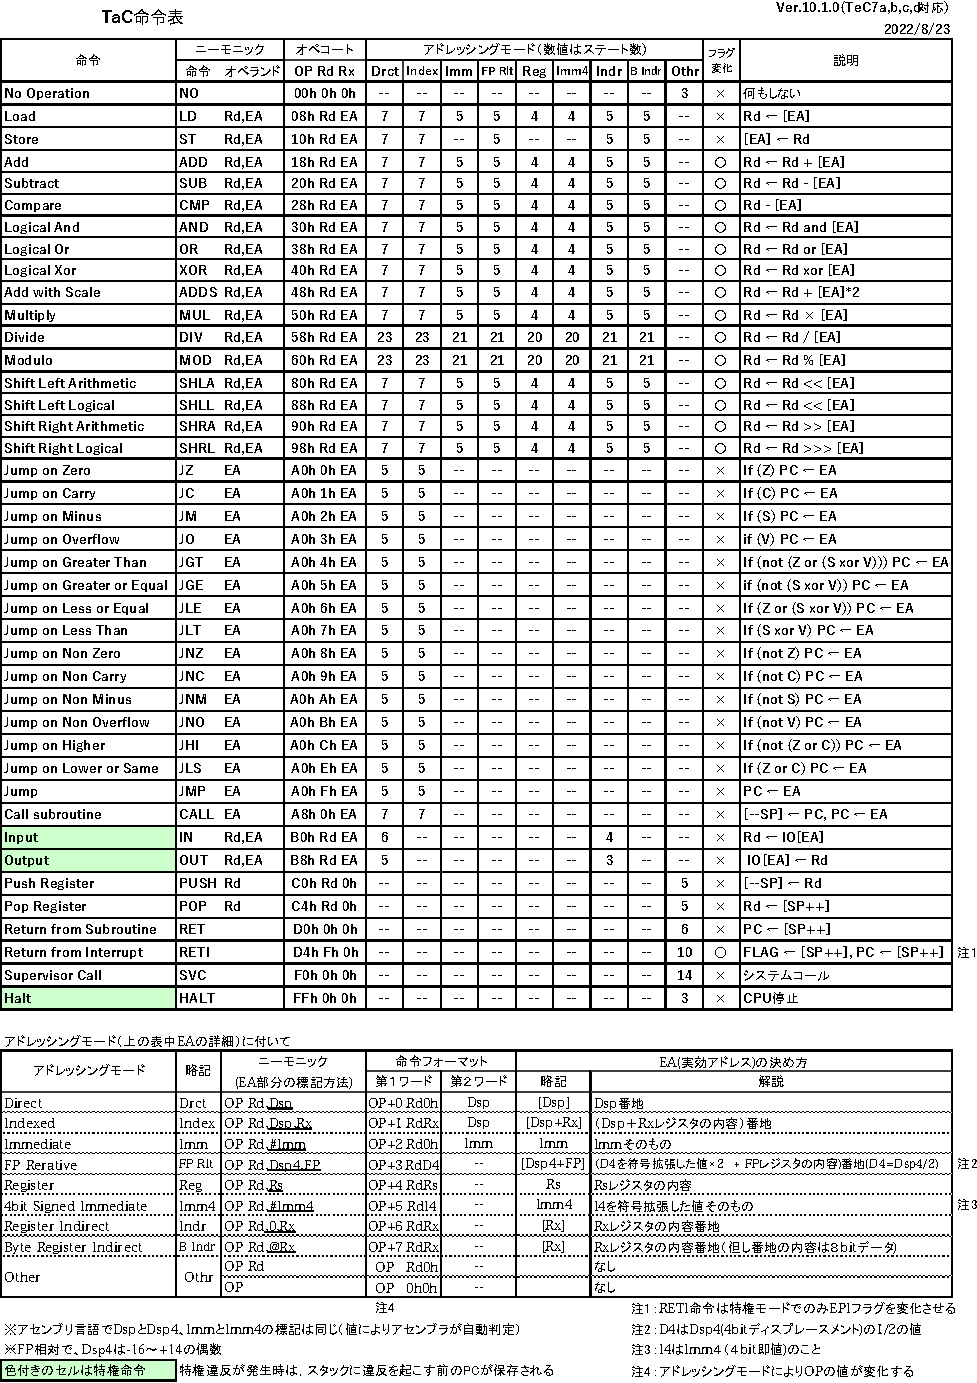
\includegraphics[scale=0.88,page=1]{Fig/TacInst-crop.pdf}
\end{myfig}

%==============================================================================
\section{機械語命令フォーマット}
TaCの機械語命令のフォーマットを\figref{tacFormat}に示す.

\begin{myfig}{p}{TaCの機械語命令フォーマット}{tacFormat}
  \includegraphics[scale=0.86,page=3]{Fig/TacInst-crop.pdf}
\end{myfig}

%==============================================================================
\section{プリント基板回路図}
TaC7dの回路図を\figref{TeC7Pcb}に示す.

\begin{myfig}{p}{TeC7dのプリント基板回路図}{TeC7Pcb}
  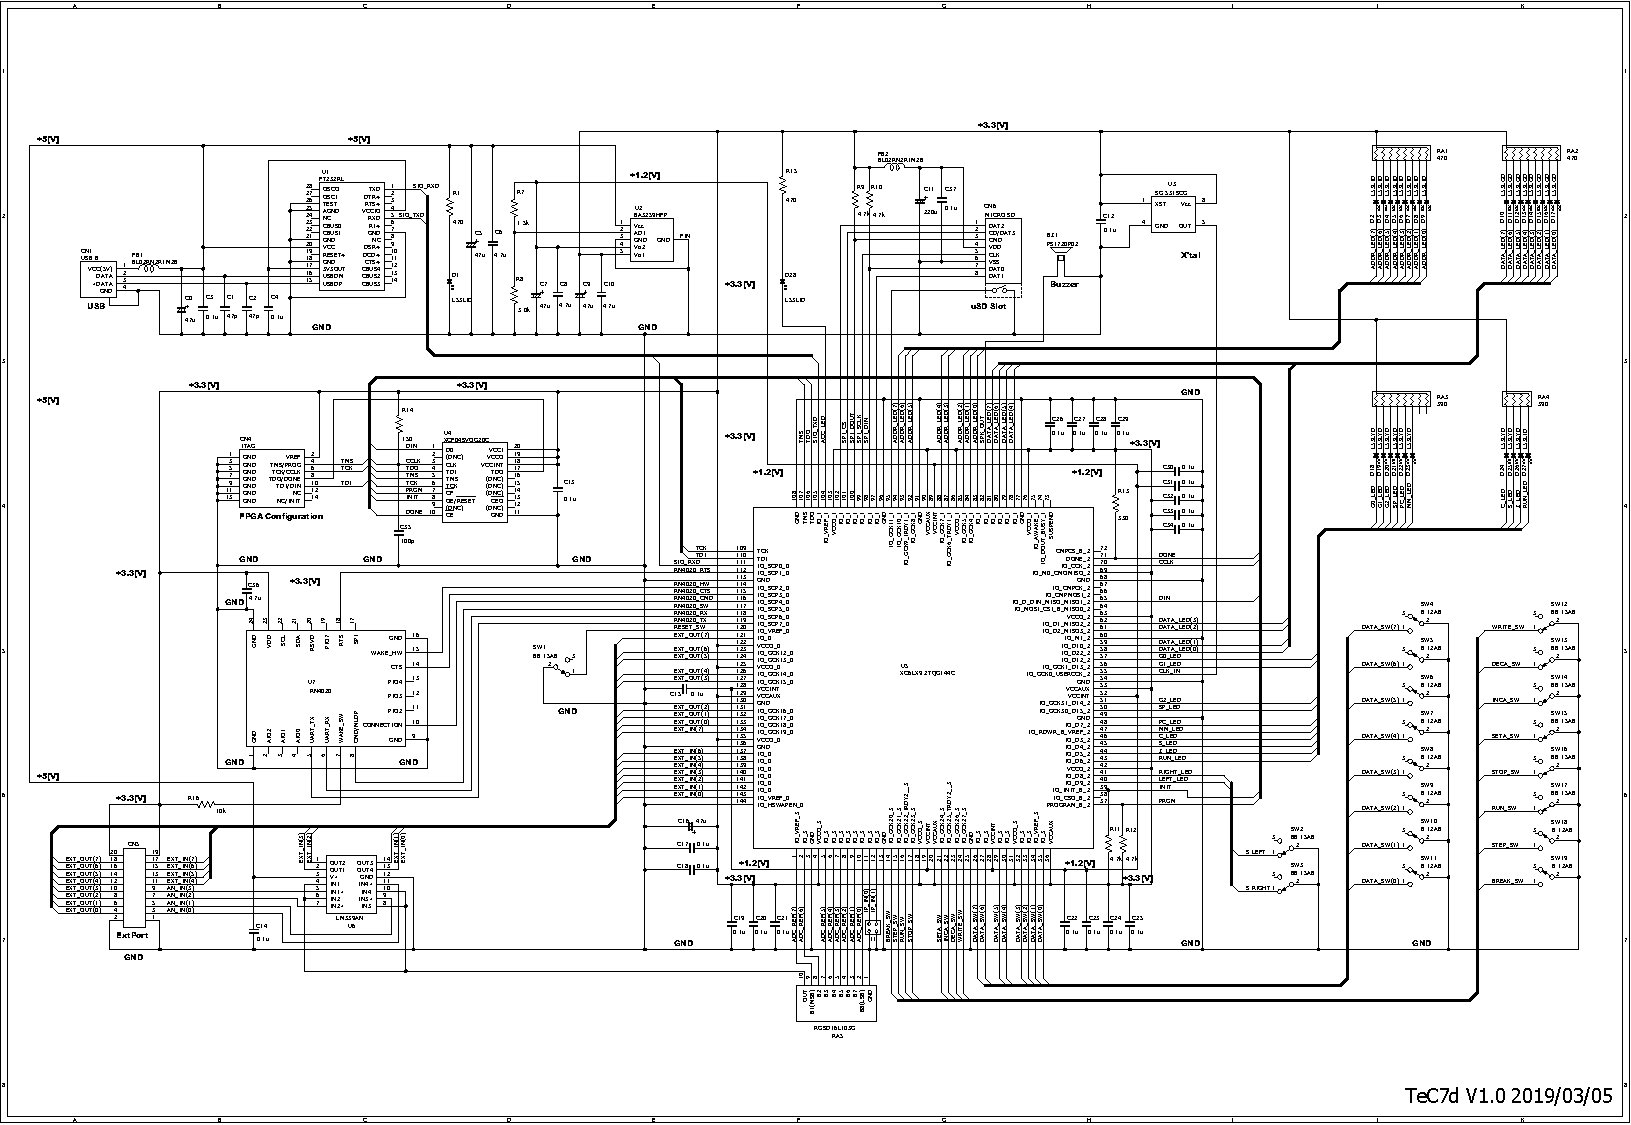
\includegraphics[angle=90,scale=0.85]{Fig/TeC7dPcb.pdf}
\end{myfig}
